\documentclass[letterpaper,notitlepage,twoside]{article}

% Basic imports, increase margins...
\usepackage[margin=0.75in]{geometry}
\usepackage{amssymb}
\usepackage{amsmath}

% Finite State Machine stuff
\usepackage{pgf}
\usepackage{tikz}
\usetikzlibrary{arrows,automata}

% Format tables nicely
\usepackage[latin1]{inputenc}
\usepackage{array}
\usepackage{booktabs}
\setlength{\heavyrulewidth}{1.5pt}
\setlength{\abovetopsep}{4pt}

\usepackage{amsfonts} 
\usepackage{amssymb}
\usepackage{amsmath,amsthm}

\renewcommand{\implies}{\Rightarrow} % redefine command "implies"  
\renewcommand{\iff}{\Leftrightarrow} % double arrow
\newcommand{\maps}{\rightarrow} % define command "map" 
\newcommand{\union}{\cup}
\newcommand{\intersect}{\cap}
\newcommand{\N}{\mathbb{N}} % natural number 
\newcommand{\Q}{\mathbb{Q}} % rational number 
\newcommand{\R}{\mathbb{R}} % real number 
\newcommand{\Z}{\mathbb{Z}} % integers 
\newcommand\tab[1][1cm]{\hspace*{#1}} %\tab command

% Add more packages that you use here...
\usepackage{graphicx}
\graphicspath{{images/}}

\begin{document}
\title{Homework 12}
\author{Joe Baker, Brett Schreiber, Brian Knotten}
\maketitle

\section*{18}
\subsection*{a}
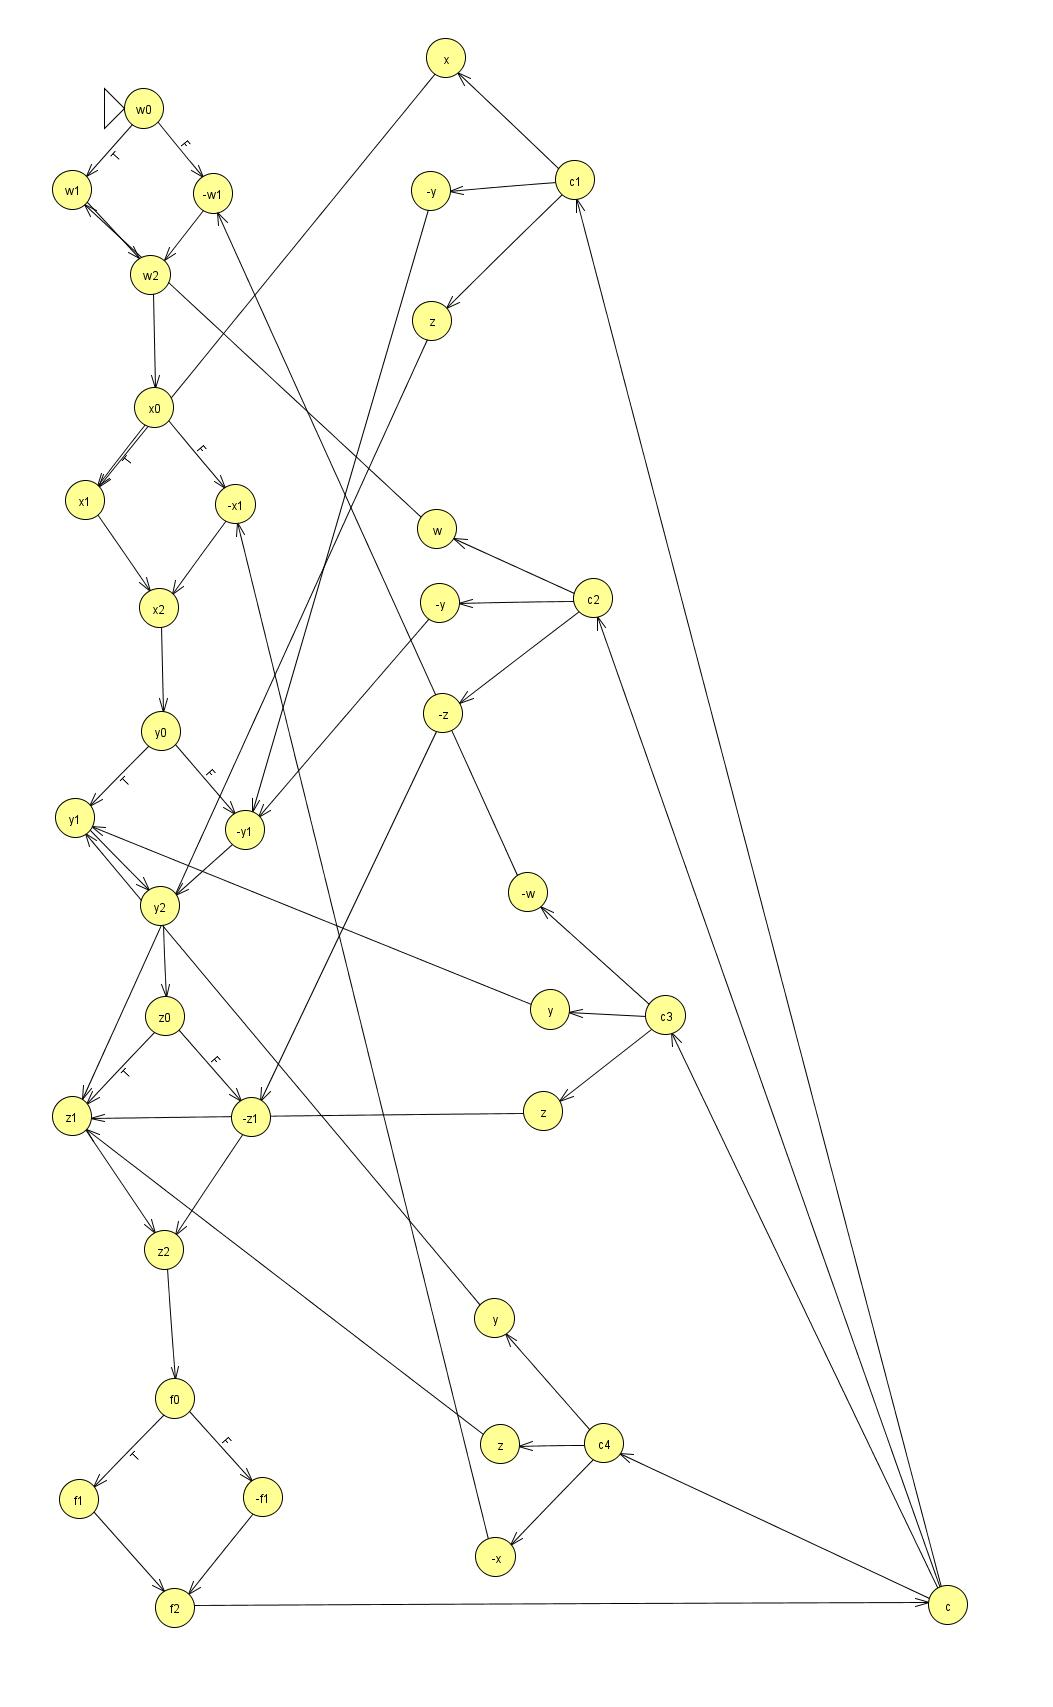
\includegraphics[scale = 0.41] {notsorted}

\subsection*{b}
The second player has a winning strategy in this instance of the Generalized Geography game, as the first player can choose in any way and still have the formula evaluate to false by the second player's choices: 
\begin{itemize}
\item If the first player sets $w=y=T$, then the second player can set $x=z=F$, causing the first clause and therefore the whole formula evaluate to false. \\
\item If the first player sets $w = F$, $y = T$, then the second player can set $z = T$ and have the second clause evaluate to false, or set $x = z = F$ and have the first clause evaluate to false. \\
\item If the first player set $w = T$, $y = F$, then the second player can set $x = T$ and $z = F$, causing both the third and fourth clauses to evaluate to false. \\
\item If the first player sets $w=y=F$, then the second player can set $x = T$ and $z = F$, causing the fourth clause to evaluate to false. \\
\end{itemize}

\end{document}

